% -*-latex-*-

\title{Orbiter Technical Notes: Nonspherical gravitational field perturbations}
\author{Martin Schweiger}
\date{September 21, 2005}

\documentclass[a4paper]{article}
\usepackage{graphicx}
\usepackage{amsmath}
\usepackage{amsfonts}
\usepackage{amssymb}
\usepackage{times}
\usepackage{cite}

\begin{document}

%\renewcommand{\vec}[1]{\ensuremath{\mathbf{#1}}}

\newcommand{\vR}[1]{\ensuremath{\vec{R}_{#1}}}
\newcommand{\nR}[1]{\ensuremath{|\vR{#1}|}}

\maketitle

\section{Introduction}
Orbiter uses a zonal representation of the gravitational potential generated by a celestial body, using a Legendre polynomial series expansion in the latitude $\theta$. The perturbations in longitude ($\phi$) are assumed to be negligible.
\begin{figure}\centering
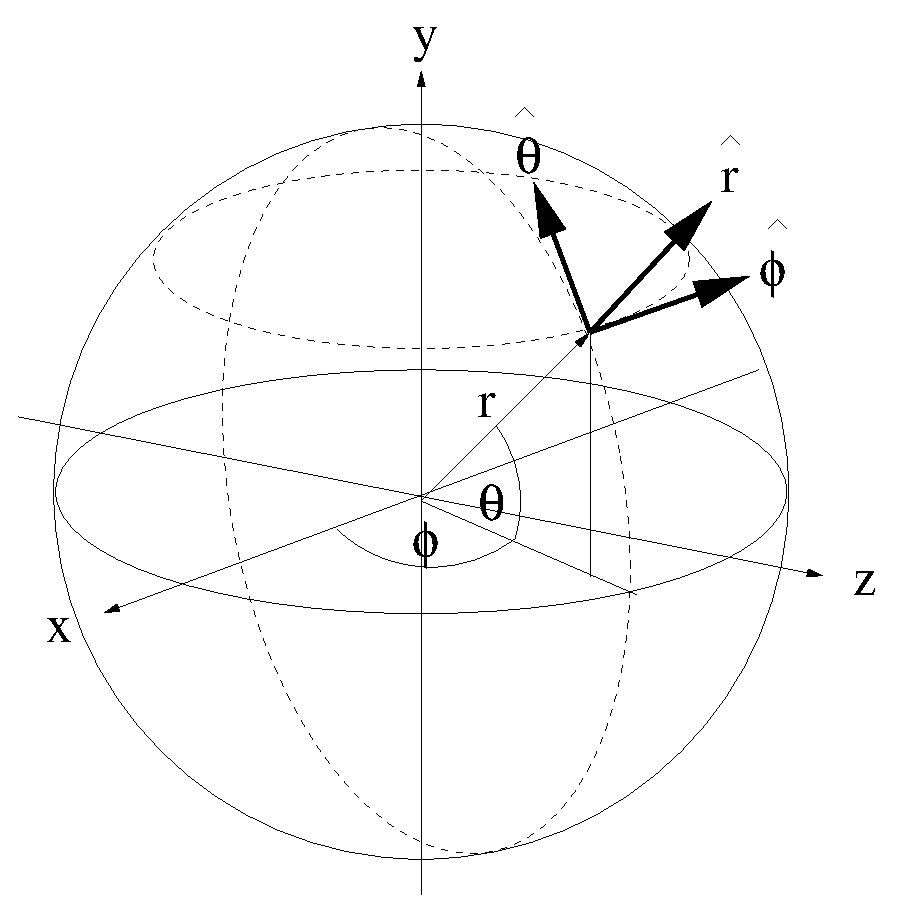
\includegraphics[width=0.45\textwidth]{sphere.eps}
\caption{Planet-relative coordinates and polar unit vectors at a point $(r,\phi,\theta)$.}
\end{figure}
The potential is expressed as
\begin{equation}\label{eq:gpot}
U_G(r,\phi,\theta) = -\frac{GM}{r} \left[ 1 - \sum_{n=2}^\infty J_n \left(\frac{R}{r}\right)^n P_n(\sin \theta) \right]
\end{equation}
where $G$ is the gravitational constant, $M$ and $R$ are the mass and mean radius of the central body, respectively, $r$ is the length of the radius vector, $J_n$ are the coefficients of the series expansion, and $P_n$ are the Legendre polynomials of order $n$.
The first Legendre polynomials are defined as
\begin{equation}
\begin{split}
P_0(x) &= 1\\
P_1(x) &= x\\
P_2(x) &= \frac{1}{2}(3x^2 - 1)\\
P_3(x) &= \frac{1}{2}(5x^3 - 3x)\\
P_4(x) &= \frac{1}{8}(35x^4 - 30x^2 +3)
\end{split}
\end{equation}
The acceleration due to the gravitational field of a test mass at point $\vec{r} = (r,\phi,\theta)$ is then given by the negative gradient of the potential:
\begin{equation}\label{eq:gacc}
\vec{a}_G(r,\phi,\theta) = -\vec{\nabla} U_G(r,\phi,\theta)
\end{equation}
In spherical polar coordinates, the gradient operator is expressed as
\begin{equation}\label{eq:polargrad}
\vec{\nabla} = \hat{r} \frac{\partial}{\partial r} + \frac{1}{r} \hat{\theta}\frac{\partial}{\partial \theta} + \frac{1}{r \cos\theta}\hat{\phi}\frac{\partial}{\partial\phi}
\end{equation}
Substituting equations \ref{eq:gpot} and \ref{eq:polargrad} into \ref{eq:gacc} yields
\begin{equation}
\vec{a}_G(r,\phi,\theta) = \hat{r} a_0^{(r)}(r) - \sum_{n=2}^\infty \left[ \hat{r} a_n^{(r)}(r,\theta) + \hat{\theta} a_n^{(\theta)}(r,\theta) \right]
\end{equation}
with the first terms given by
\begin{equation}
\begin{split}
a_0^{(r)}(r) &= -\frac{GM}{r^2} \\
a_2^{(r)}(r,\theta) &= -\frac{3}{2} \frac{GMR^2 J_2}{r^4}(3\sin^2\theta - 1)\\
a_2^{(\theta)}(r,\theta) &= 3 \frac{GMR^2 J_2}{r^4} \sin\theta \cos\theta \\
a_3^{(r)}(r,\theta) &= -2 \frac{GMR^3 J_3}{r^5}(5 \sin^3\theta - 3\sin\theta)\\
a_3^{(\theta)}(r,\theta) &= \frac{3}{2} \frac{GMR^3 J_3}{r^5} (5 \sin^2\theta \cos\theta - \cos\theta) \\
a_4^{(r)}(r,\theta) &= -\frac{5}{8} \frac{GMR^4 J_4}{r^6}(35 \sin^4\theta - 30\sin^2\theta + 3) \\
a_4^{(\theta)}(r,\theta) &= \frac{5}{2} \frac{GMR^4 J_4}{r^6} (7 \sin^3\theta \cos\theta - 3 \sin\theta \cos\theta)
\end{split}
\end{equation}
The coefficients $J_n$ used by Orbiter are listed in Table~\ref{tab:Jn}.
\begin{table}
\begin{tabular}{lcccc}
        & $J_2$     & $J_3$ & $J_4$ & $J_5$ \\ \hline
Mercury & 60        & -     & -     & -     \\
Venus   & 27        & -     & -     & -     \\ 
Earth   & 1082.6269 & -2.51 & -1.60 & -0.15 \\
Mars    & 1964      & -     & -     & -     \\
Jupiter & 14750     & -     & -     & -     \\
Saturn  & 16450     & -     & -     & -     \\
Uranus  & 12000     & -     & -     & -     \\
Neptune & 4000      & -     & -     & -
\end{tabular}
\caption{Coefficients ($\times 10^6$) for zonal expansion of planetary gravitational potentials.}
\label{tab:Jn}
\end{table}

The field perturbations can lead to a rotation of the orbit trajectory of a satellite. This rotation can be expressed in terms of the movement of the longitude of the ascending node ($\Omega$) and the movement of the argument of periapsis ($\omega$).
If only terms up to $J_2$ are included, approximate values of the movements $\partial\Omega/\partial t$ and $\partial\omega/\partial t$ are given by
\begin{eqnarray}
\frac{\partial\Omega}{\partial t} &=& -\frac{3 n}{2} \left(\frac{R}{a}\right)^2 \frac{\cos i}{(1-e^2)^2} J_2 \label{eq:noderate} \\
\frac{\partial\omega}{\partial t} &=& \frac{3 n}{4} \left(\frac{R}{a}\right)^2 \frac{5 \cos^2 i - 1}{(1-e^2)^2} J_2
\end{eqnarray}
where $n=2\pi/P$ is the mean motion (with orbit period $P$), $a$ is the mean distance, $e$ is the eccentricity, and $i$ is the inclination.

\subsection*{Example: calculate the inclination for a sun-synchronous polar orbit}
A sun-synchronous orbits exploits the propagation of the line of nodes to keep the orbital plane synchronised with the relative position of the sun. A satellite can for example be placed in a sun-synchronous orbit so that it continuously flys over the planet's terminator line.
From~\ref{eq:noderate} we have
\begin{equation}
\cos i = -\frac{2}{3 n} \left(\frac{a}{R} \right)^2 \frac{(1-e^2)^2}{J_2} \frac{\partial\Omega}{\partial t}
\end{equation}
A sun-synchronous orbit requires the line of nodes to move at a rate of $2\pi$ per year. For Earth, this is equivalent to $\partial\Omega/\partial t = 1.99\cdot 10^{-7}$\,rad/s (about $0.99$ deg. per day). Assume a circular orbit ($e=0$) at an altitude of 300\,km
%($a = 6 678 137$\,m, with $R_E = 6 378 137$\,m).
($a = 6 671 010$\,m, with $R_E = 6 371 010$\,m).
With $P = 2\pi\sqrt{a^3/\mu_E}$ we get $n = \sqrt{\mu_E/a^3} = 0.0012$\,rad/s. This leads to
\begin{equation}
\cos i_\text{sync} = -\frac{2}{0.0035} \left(\frac{6 678 137}{6 378 137}\right)^2 \frac{1.99\cdot 10^{-7}}{0.001082630} = -0.116,
\end{equation}
or $i_\text{sync} = 96.7$\,deg.
\end{document}
